\documentclass[border=5mm]{standalone}
\usepackage{tikz}
\usepackage{pgffor}
\usetikzlibrary{calc}
\usetikzlibrary{decorations.pathreplacing}
\usetikzlibrary{positioning,shapes,arrows,arrows.meta}
\tikzstyle{startstop} = [draw, rounded rectangle, text centered, draw=black,thick]
\tikzstyle{io} = [trapezium, trapezium left angle=70, trapezium right angle=110, text centered, draw=black,thick]
\tikzstyle{process} = [rectangle, text centered, draw=black,thick]
\tikzstyle{decision} = [diamond, text centered, draw=black,thick]
\tikzstyle{arrow} = [-{Stealth[scale=1.2]},rounded corners,thick]

\newsavebox{\tempbox}
\newcommand{\textbox}[1]% #1 = text
{\savebox{\tempbox}{#1}% get width
	\ifdim\wd\tempbox<6cm\relax
	\makebox[6cm]{\usebox{\tempbox}}%
	\else
	\parbox{6cm}{\raggedright #1}%
	\fi}
\begin{document}
	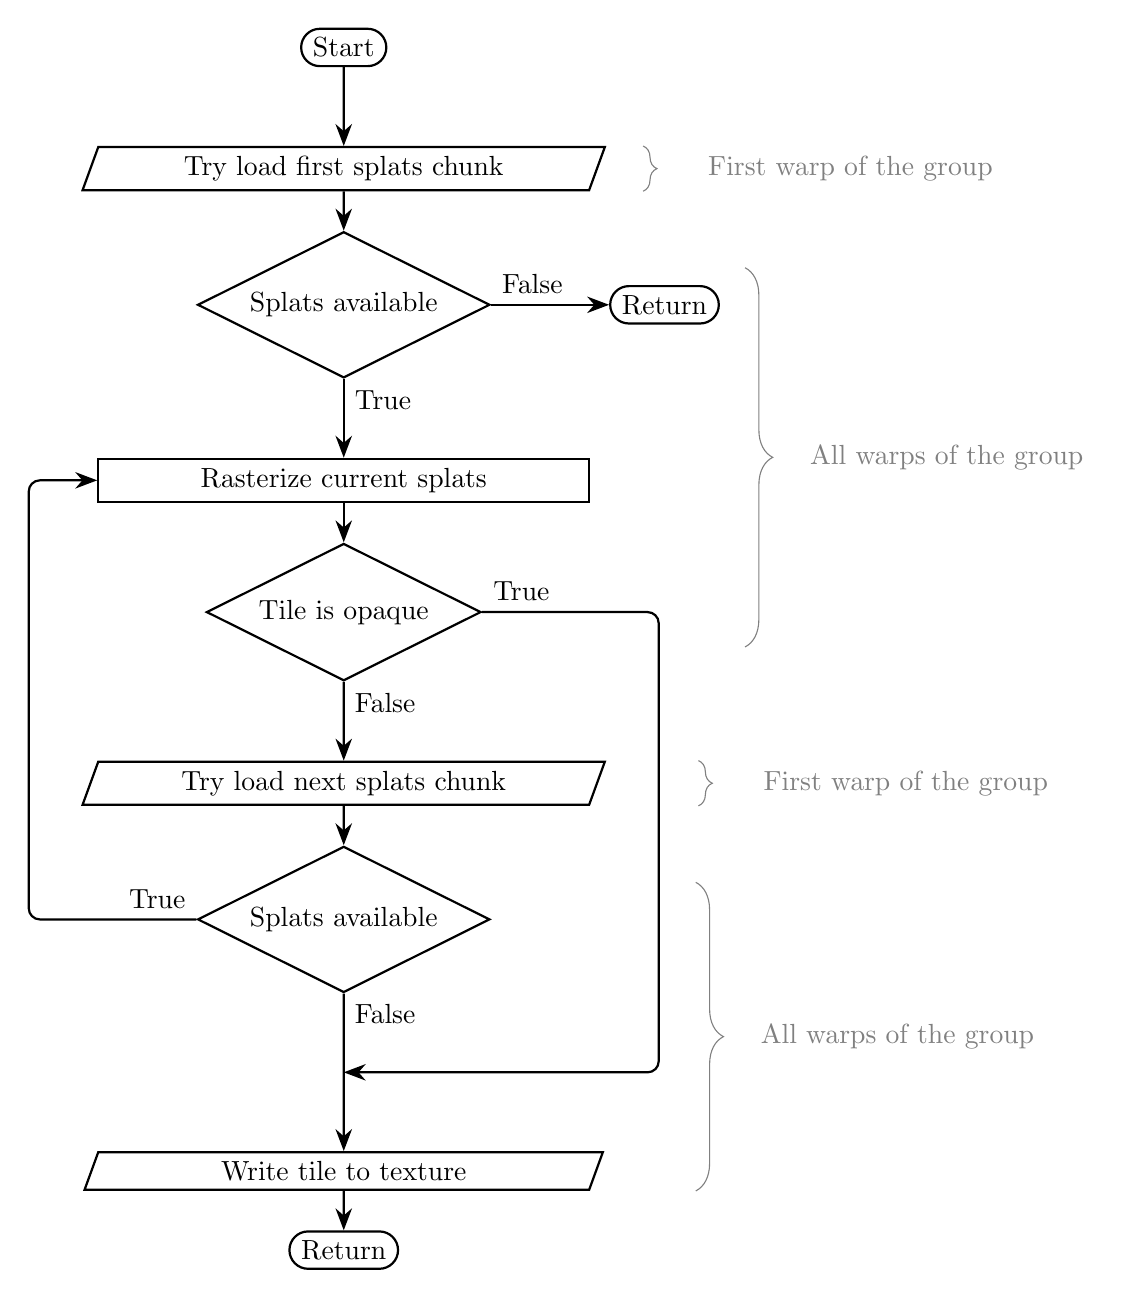
\begin{tikzpicture}
		\node (start) [startstop] {Start};
		\node (load-splats) [io,below=1.0 of start] {\textbox{Try load first splats chunk}};
		\node (exit-if-empty) [decision,aspect=2,below=0.5 of load-splats] {Splats available};
		\node (return) [startstop,right=1.5 of exit-if-empty] {Return};
		\node (rasterize) [process,below=1.0 of exit-if-empty] {\textbox{Rasterize current splats}};
		\node (exit-if-opaque) [decision,aspect=2,below=0.5 of rasterize] {Tile is opaque};
		\node (load-splats-2) [io,below=1.0 of exit-if-opaque] {\textbox{Try load next splats chunk}};
		\node (exit-if-no-splats) [decision,aspect=2,below=0.5 of load-splats-2] {Splats available};
		\node (write-tile) [io,below=2.0 of exit-if-no-splats] {\textbox{Write tile to texture}};
		\node (return2) [startstop,below=0.5 of write-tile] {Return};
		
		\draw [arrow] (start) --  (load-splats);
		\draw [arrow] (load-splats) --  (exit-if-empty);
		\draw [arrow] (exit-if-empty) --  (return);
		\draw [arrow] (exit-if-empty) --  (rasterize);
		\draw [arrow] (rasterize) --  (exit-if-opaque);
		\draw [arrow] (exit-if-opaque) --  (load-splats-2);
		\draw [arrow] (load-splats-2) --  (exit-if-no-splats);
		\draw [arrow] (exit-if-no-splats) --  coordinate[midway](m1)(write-tile);
		\draw [arrow] (write-tile) -- (return2);
		
		\draw [arrow] (exit-if-opaque) -- + (4.0,0) |- (m1);
		\draw [arrow] (exit-if-no-splats) -- + (-4.0,0) |- (rasterize.west);
		
		\node [black,above right =0.05em and 0.05em of exit-if-empty.east] {False};
		\node [black,below right =0.05em and 0.05em of exit-if-empty.south] {True};
		\node [black,below right =0.05em and 0.05em of exit-if-opaque.south] {False};
		\node [black,above right =0.05em and 0.05em of exit-if-opaque.east] {True};
		\node [black,below right =0.05em and 0.05em of exit-if-no-splats.south] {False};
		\node [black,above left =0.05em and 0.05em of exit-if-no-splats.west] {True};
		
		\draw [gray, decorate,decoration={brace, raise=10.0em, amplitude=0.5em}] 
		let \p1=(load-splats.north east) in (\x1,\y1)
		let \p2=(load-splats.south east) in (\x2,\y2)
		(\x2,\y1) -- (\x2,\y2) node[pos=0.5,right=12.0em,gray]{First warp of the group};
		
		\draw [gray, decorate,decoration={brace, raise=12.0em, amplitude=1.0em}] 
		let \p1=(exit-if-empty.north east) in (\x1,\y1)
		let \p2=(exit-if-opaque.south east) in (\x2,\y2)
		(\x2,\y1) -- (\x2,\y2) node[pos=0.5,right=14.0em,gray]{All warps of the group};
		
		\draw [gray, decorate,decoration={brace, raise=12.0em, amplitude=0.5em}] 
		let \p1=(load-splats-2.north east) in (\x1,\y1)
		let \p2=(load-splats-2.south east) in (\x2,\y2)
		(\x2,\y1) -- (\x2,\y2) node[pos=0.5,right=14.0em,gray]{First warp of the group};
		
		\draw [gray, decorate,decoration={brace, raise=12.0em, amplitude=1.0em}] 
		let \p1=(exit-if-no-splats.north east) in (\x1,\y1)
		let \p2=(write-tile.south east) in (\x2,\y2)
		(\x2,\y1) -- (\x2,\y2) node[pos=0.5,right=14.0em,gray]{All warps of the group};
		
	\end{tikzpicture}
\end{document}